% Document principal LaTeX pour compte-rendu
\documentclass[12pt]{report}
\usepackage{BidoTexCourses}
\usepackage{hyperref}
\usepackage{graphicx}


\title{Compte rendu projet Portal 0.0}
\author{BIDAULT Matthieu, BADSTÜBER Elian, FOCHEUX Vital}
\date{\today}

\renewcommand{\contentsname}{
	Table des matières
}

\begin{document}

\maketitle

\section*{Remerciements}

\paragraph{}
Nous tenons à remercier notre enseignant de projet, M. \textsc{Bernard} 
qui a su nous guider et nous conseiller tout au long de ce projet.


\tableofcontents

\section{Introduction}

\paragraph{}

Dans le cadre du projet semestriel de troisième année de licence
informatique à l'université de Franche-Comté, nous proposons de coder
une version très simplifiée du jeu \href{https://fr.wikipedia.org/wiki/Portal_(jeu_vid%C3%A9o)}{Portal}
qui sera afficher grâce à un moteur de type Raycaster à la façon du jeu
\href{https://fr.wikipedia.org/wiki/Wolfenstein_3D}{Wolfenstein 3D}.
Il a pour but de nous faire découvrir le monde du développement de jeux 
vidéo en nous faisant réaliser un jeu vidéo en C++ avec la bibliothèque 
GF.

% \clearpage

\section{Besoins et objectifs du projet}
\subsection{Contexte}

\begin{figure}[H]
    \begin{minipage}{0.48\textwidth}
		% \centering
        \paragraph{Les graphismes : }
		Au début des années 90, la société \href{https://fr.wikipedia.org/wiki/Id_Software}{Id Software} a entrepris des 
		recherches pionnières dans le domaine des graphismes 3D, alors principalement réservés aux simulateurs de vols tels 
		que \href{https://fr.wikipedia.org/wiki/Wing_Commander_(jeu_vid%C3%A9o)}{Wing Commander} ou 
		\href{https://en.wikipedia.org/wiki/Knights_of_the_Sky}{Knights of the Sky}, deux titres parus en 1990. Face aux 
		contraintes de performance des ordinateurs de l'époque, le développement de jeux d'action en 3D rapide représentait 
		un défi de taille. 
    \end{minipage}\hfill
    \begin{minipage}{0.48\textwidth}
        \centering
        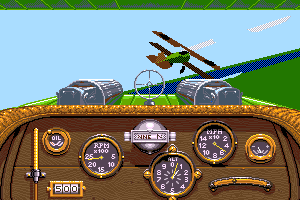
\includegraphics[width=\linewidth]{image/knights-of-the-sky.png}
		\hspace*{-0.5cm}
        \caption{Knights of the Sky}
        \label{fig:knights-of-the-sky}
    \end{minipage}
\end{figure}

\begin{figure}[H]
	\begin{minipage}{0.48\textwidth}
		\centering
		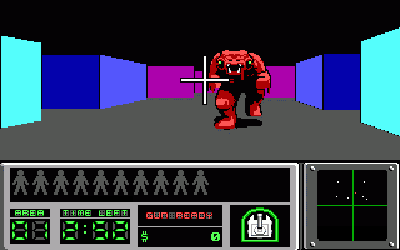
\includegraphics[width=\linewidth]{image/Hovertank_3D.png}
		\hspace*{-0.5cm}
		\caption{Hovertank 3D}
		\label{fig:hovertank3d}
	\end{minipage}\hfill
	\begin{minipage}{0.48\textwidth}
		% \centering
		C'est dans ce contexte que \href{https://fr.wikipedia.org/wiki/John_Carmack}{John Carmack} a 
		proposé l'utilisation de la technique du \href{https://fr.wikipedia.org/wiki/Raycasting}{raycasting}, permettant 
		de calculer uniquement les surfaces visibles par le joueur. En six semaines, Carmack développe un moteur 3D innovant 
		utilisant des sprites 2D pour représenter les entités du jeu. Ce moteur a été utilisé dans le jeu 
		\href{https://fr.wikipedia.org/wiki/Hovertank_3D}{Hovertank 3D}, publié en avril 1991.
	\end{minipage}
\end{figure}

\begin{figure}[H]
	\begin{minipage}{0.48\textwidth}
		À l'automne 1991, alors que \href{https://fr.wikipedia.org/wiki/John_Carmack}{John Carmack} et 
		\href{https://fr.wikipedia.org/wiki/John_Romero}{John Romero} finalisaient le moteur de 
		\href{https://en.wikipedia.org/wiki/Commander_Keen_in_Goodbye,_Galaxy}{Commander Keen in Goodbye, Galaxy}, Carmack 
		découvre \href{https://fr.wikipedia.org/wiki/Ultima_Underworld}{Ultima Underworld}, un jeu développé par 
		\href{https://fr.wikipedia.org/wiki/Looking_Glass_Studios}{Blue Sky Productions} (qui deviendra plus tard Looking Glass Studios), 
		doté d'un moteur capable de rendre des graphismes 3D 
		texturés sans subir les limitations de Hovertank 3D.
	\end{minipage}\hfill
	\begin{minipage}{0.48\textwidth}
		\centering
		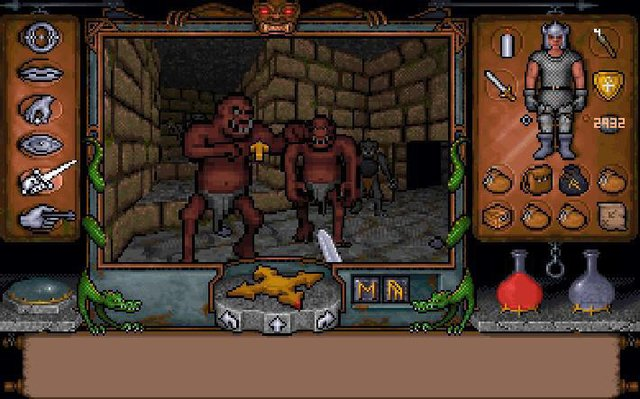
\includegraphics[width=\linewidth]{image/Ultima_Underworld.jpg}
		\hspace*{-0.5cm}
		\caption{Ultima Underworld}
		\label{fig:ultimaunderworld}
	\end{minipage}
\end{figure}

\begin{figure}[H]
	\begin{minipage}{0.48\textwidth}
		\centering
		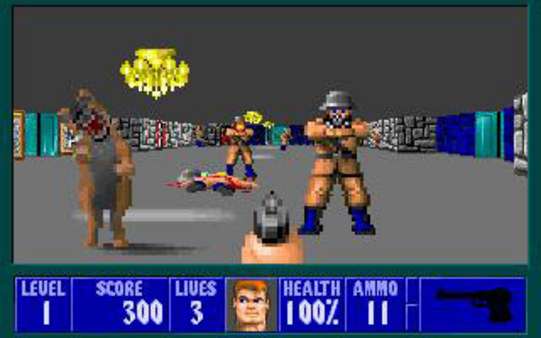
\includegraphics[width=\linewidth]{image/wolfenstein_3d.jpg}
		\hspace*{-0.5cm}
		\caption{Wolfenstein 3D}
		\label{fig:wolfenstein3d}
	\end{minipage}\hfill
	\begin{minipage}{0.48\textwidth}
		Inspiré, Carmack décide d'améliorer son propre moteur pour 
		intégrer le mapping de textures tout en conservant de hautes performances. Après un intense travail de six semaines, 
		le nouveau moteur 3D est achevé et utilisé pour le jeu \href{https://fr.wikipedia.org/wiki/Catacomb_3D}{Catacomb 3D},
		publié en novembre 1991. La révélation de Catacomb 3D a poussé 
		\href{https://fr.wikipedia.org/wiki/Scott_Miller_(programmeur)}{Scott Miller} d'Apogee à convaincre l'équipe de 
		développer un jeu d'action en 3D sous forme de shareware. Cela a conduit au lancement du projet 
		\href{https://fr.wikipedia.org/wiki/Wolfenstein_3D}{Wolfenstein 3D}, un remake en 3D de 
		\href{https://fr.wikipedia.org/wiki/Castle_Wolfenstein}{Castle Wolfenstein}. Sorti le 5 mai 1992 sur PC, ce jeu a 
		non seulement été un succès commercial mais a également posé les bases du genre du jeu de tir à la première personne, 
		préfigurant ainsi des titres légendaires tels que 
		\href{https://fr.wikipedia.org/wiki/Doom_(jeu_vid%C3%A9o,_1993)}{Doom} et 
		\href{https://fr.wikipedia.org/wiki/Quake}{Quake}.
	\end{minipage}
\end{figure}

% \begin{figure}[H]
%     \begin{minipage}{0.48\textwidth}
%         \centering
%         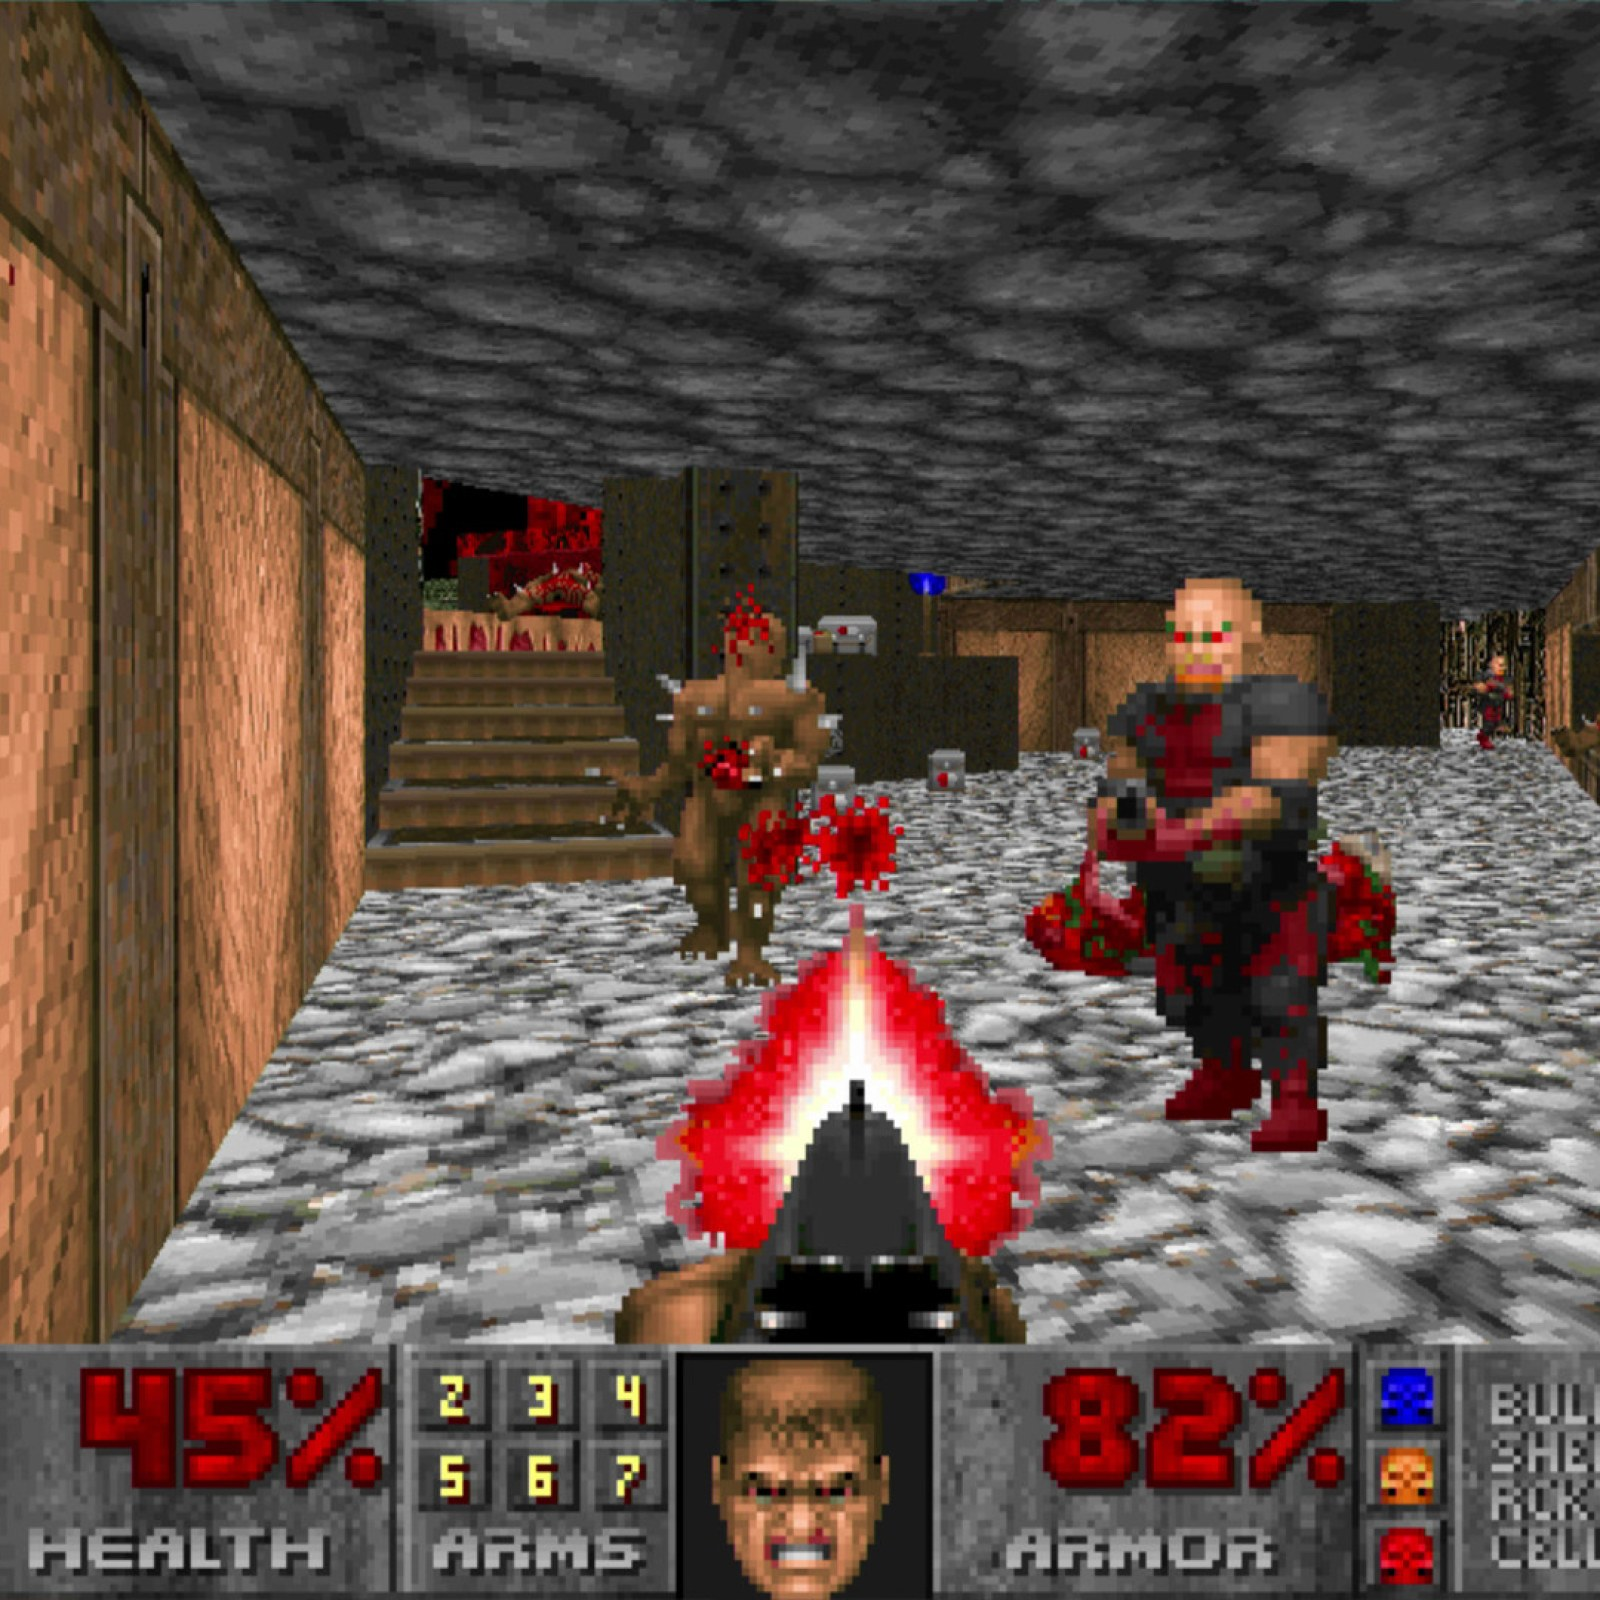
\includegraphics[width=\linewidth]{image/doom_1993.jpg}
%         \caption{Doom (1993)}
%         \label{fig:doom1993}
%     \end{minipage}\hfill
%     \begin{minipage}{0.48\textwidth}
%         \centering
%         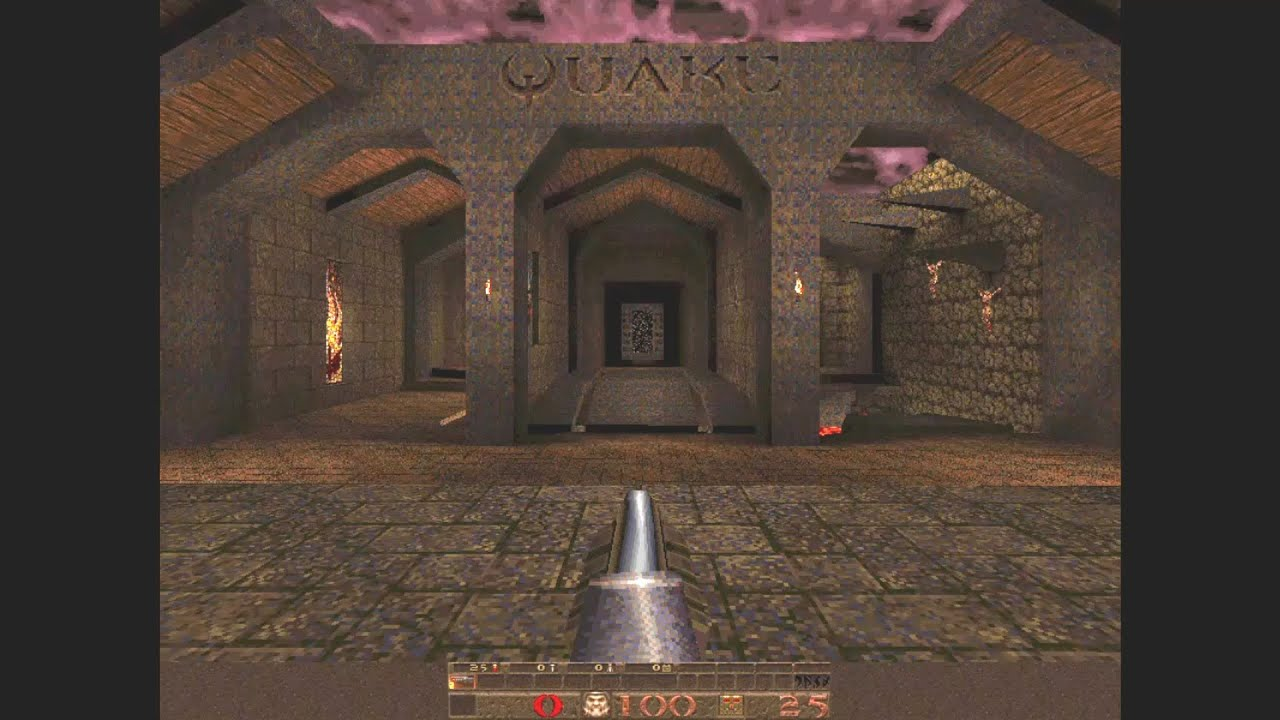
\includegraphics[width=\linewidth]{image/quake_1996.jpg}
%         \caption{Quake (1996)}
%         \label{fig:quake1996}
%     \end{minipage}
% \end{figure}

% \begin{figure}[h]
% 	\centering
% 	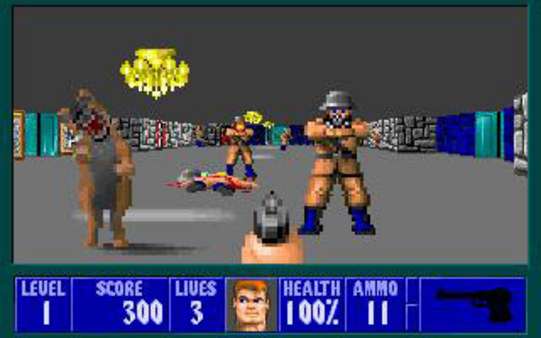
\includegraphics[width=0.5\textwidth]{image/wolfenstein_3d.jpg}
% 	\caption{Wolfenstein 3D}
% 	\label{fig:wolfenstein3d}
% \end{figure}






\begin{figure}[H]
	\paragraph{Le système de jeu : }
	En 2007, \href{https://fr.wikipedia.org/wiki/Valve_Corporation}{Valve Corporation} a révolutionné le genre des jeux 
	de réflexion à la première personne avec la sortie de 
	\href{https://fr.wikipedia.org/wiki/Portal_(jeu_vid%C3%A9o)}{Portal}. Ce jeu introduit un mécanisme unique 
	permettant au joueur de générer deux portails, l'un orange et l'autre bleu, sur des surfaces planes et 
	interconnectées. Ces portails offrent la possibilité de traverser instantanément l'espace d'un point à un autre, 
	tout en conservant l'inertie. L'objectif est de résoudre divers puzzles en se servant de cette capacité à manipuler 
	l'espace pour atteindre la sortie des différents niveaux proposés.
	\begin{figure}[H]
		\centering
		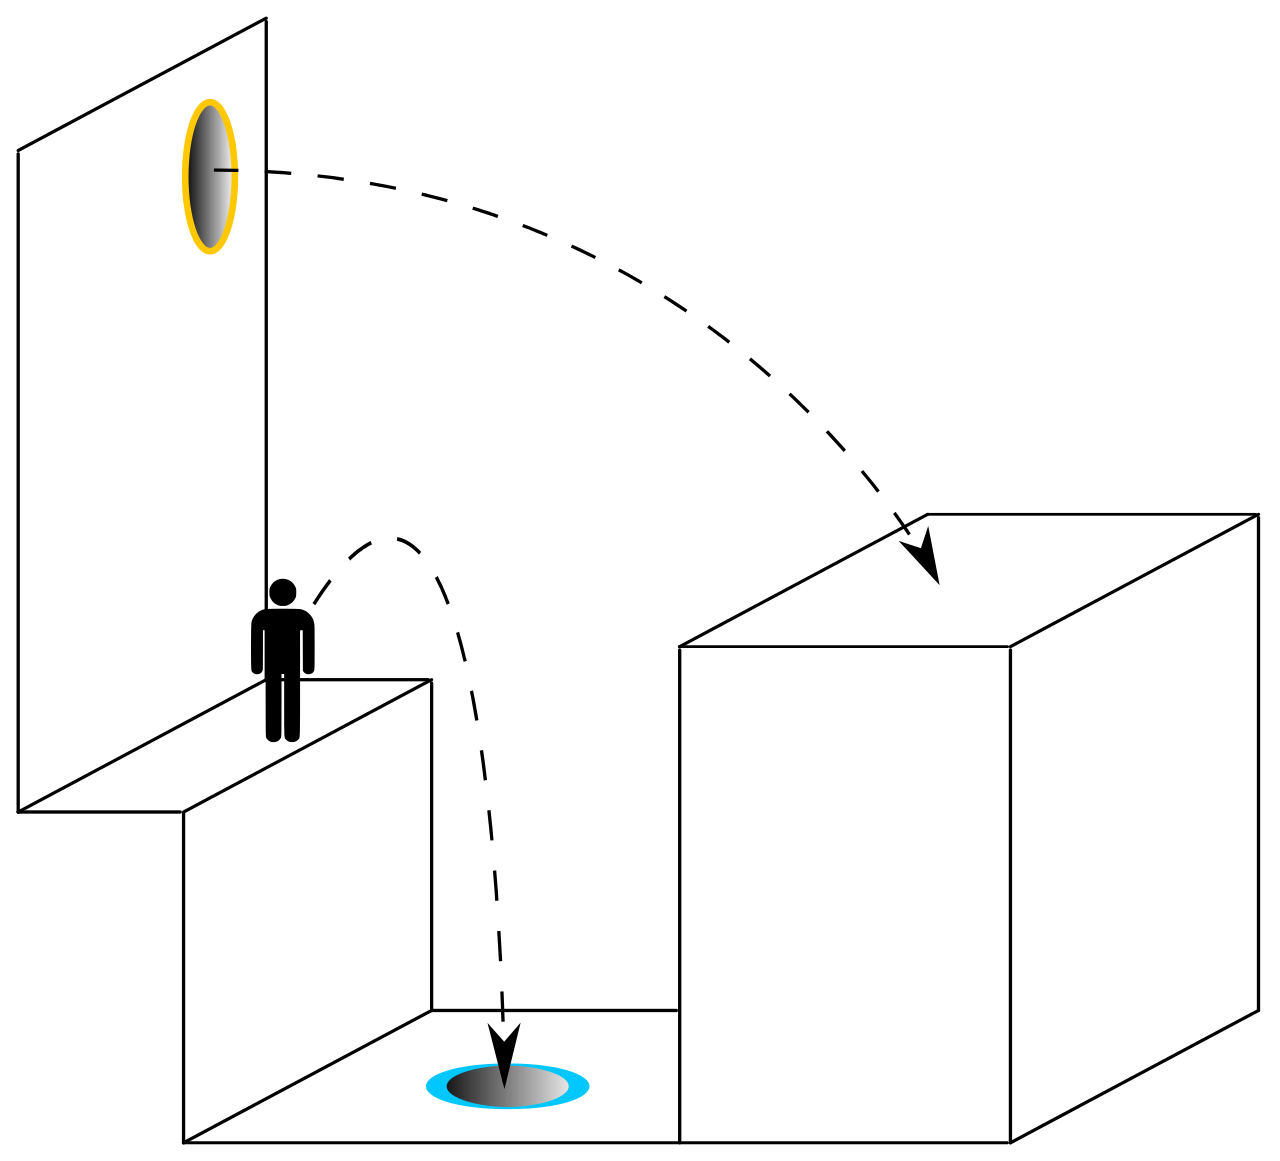
\includegraphics[width=0.5\textwidth]{image/schema_portal.png}
		\hspace*{-0.5cm}
		\caption{Schéma de fonctionnement du système de portail}
		\label{fig:schema_portal}
	\end{figure}
\end{figure}
% \clearpage

\subsection{Motivations}

\paragraph{}

L'une des motivations principales de ce projet est de réaliser un jeu vidéo
avec graphique comme à l'époque de \href{https://fr.wikipedia.org/wiki/Wolfenstein_3D}{Wolfenstein 3D} 
mais avec des comcepts de jeux plus récentes et qui plus est pourrai être
un préquel de \href{https://fr.wikipedia.org/wiki/Portal_(jeu_vid%C3%A9o)}{Portal}.


\subsection{Objectif et contraintes}

\paragraph{}
Les principaux objectifs de ce projet sont :
\begin{itemize}
	\item Réaliser un jeu vidéo en C++ avec la bibliothèque GF
	\item Implémenter un moteur de type Raycaster
	\item Implémenter un système de portail
	\item Implémenter un système de collision
	\item Offir une expérience de jeu simple et agréable à jouer.
\end{itemize}

\paragraph{}
Mais avec des contraintes :
\begin{itemize}
	\item L'apprentissage d'un langage de programmation nouveau pour nous
	\item L'apprentissage d'une bibliothèque de programmation nouvelle pour nous
	\item L'apprentissage de la programmation d'un moteur de type Raycaster
	\item L'apprentissage de la programmation d'un système de portail
	\item L'apprentissage de la programmation d'un système de collision
	\item L'apprentissage de la programmation d'un système de jeu
\end{itemize}

\section{Gestion du projet}
\subsection{L'équipe}
\subsection{Planification et outils de gestion}

\paragraph{}
Pour la gestion du projet nous avons utilisé le site 
\href{https://github.com/}{github} qui est un outil de gestion 
de projet en ligne.

\subsection{Répartition des tâches}

\section{Développement}
\subsection{Différentes stratégie}
\subsection{Programmer en C++}
\subsection{Apprendre à utiliser la bibliothèque GF}

\section{Bilan du projet}
\subsection{Résultats obtenus}
\subsection{Apports technique}
\subsection{Apports personnels}

\section{Perspectives}
\subsection{Améliorations possibles}
\subsection{Nouvelles fonctionnalités}
\subsection{Un plus dans nos CV}

\section{Bibliographie}


\end{document}